% !TEX root = ../thesis_main.tex
\chapter{Materials and Methods}\label{chap:MaterialsAndMethods}
    \section{Parahydrogen generation and quantification}
    Parahydrogen was generated using a coldhead surrounding a chamber of $\mathrm{FeO_4}$ catalyst which was built before the beginning of this work. 
        \subsection{Coldhead side}
            The coldhead was cooled down to \SI{21}{\kelvin} via a watercooled helium recondenser with a closed helium circuit. The recondenser was operated at full power while a heater was installed to keep temperatures at 21 K. The coldhead was isolated from surrounding warm air by a vacuum chamber pumped down by a rotary vane pump. A sensor attached to the vaccum chamber read pressures to ensure sufficient isolation before switching on the recondenser. Temperature sensors in the catalyst chamber and on top of the coolant line were used for checking whether the conversion can be started and also as a feedback for the heater to regulate temperature.
        \subsection{Hydrogen side}
        The system was usually flooded with nitrogen gas before use to ensure that no explosive mixtures could built. As the nitrogen freezing point is at \SI{}{\kelvin}, it needed to be removed before cooling though. This was done by flushing the system with hydrogen gas. The system consisted of the hydrogen and nitrogen supply bottles (\SI{10}{\liter}, \SI{200}{\bar}, 99.999\% pure), both with individual pressure regulators and additional cutoff valves. The lines from the supply bottles then combine into a single line running towards and trough the coldhead and its catalyst chamber where the conversion occurs. Behind that coldhead, a needle valve regulates flow and can be switched between a flow meter to measure and set the flow against atmospheric pressure and a bottle storing the parahydrogen. Pressure limits given by the manufacturer are \SI{50}{\bar}. 
    \section{Low field NMR}
        To acquire NMR spectra at fields where 1H-Sabre is feasible \todo{Ref sabre}, a low field NMR
        spectrometer was built \todo{ref niels} previous to this work. Its main field is generated by a resisitve
        coil in solenoid or dual helmholtz assembly design. Inside that coil, there is a saddle coil
        generating a $B_1$ field perpendicular to $B_0$. Inside and perpendicular to both, a third
        coil, usually a solenoid, is used to detect the signal generated through the spin manipulation.
        \subsection{Static magnetic field}
            Multiple coil designs of the static field generating coils have been  considered, simulated, built and tested in the course of this work. The previously used solenoid design with different lengths of compensation windings \ref{simulation:B0} showed to have disadvantages over the dual helmholz asssembly built during this work.
        \subsubsection{Solenoid coil}
            The $B_0$ coil is wound around an acrylic tube in two full layers. In addition, at the
            tube's ends, compensation windings are installed to homogenize the field inside the coil.
            The length of these windings was optimized in matlab simulations \ref{} \todo{figure of whole setup}
            Coils ususally consist of one or more layers of wire usually wound around a PVC tube. Spacing between layers is given by wire thickness including insulation. To keep  these distances small and, in turn, magnetic flux density high, enameled wire was used for all coils. Winding of the wire was mostly performed on a turning lathe enabling automatic counting of the number of windings and a steady, cosistent feed of the wire.
            The solenoid coil used in the main low field experiments consisted of a three layered solenoid with two layers of compensation windings on each side. The main layers consisted of NN windings with an inner diameter of \SI{130}{\mm}. The overall length is \SI{350}{\milli\meter}.
        \subsubsection{Helmholtz coil}
            To build a homogeneous dual helmholtz array, simulations were also considered. as space was limited inside the Mu metal shield the coil was also supposed to be used in, the coils' diameters were predetermined and only the coils distances and currents were optimized (see \ref{simulations:B0} for details). As the general setup, a PVC tube onto which four coil holders  were mounted was chosen. Using the simulation results, a layout for the coil holders was designed. To keep unwanted fields due to connecting wires to a minimum, these wires were kept as short as possible. Holders were lathed and then processed further by hand. Winding of the wire was also done by hand. To keep the wire form sliding into the gouges of the previous layer, PVC foil was lasercut to fit the dimensions of the coil holders. Due to the limited size of the foil used (Din A4) and the relatively large diameter of the coils, three stripes of foil were connected with one of the three parts employing a feedthrough for the wire transversing from one layer to the next. 
        \subsection{Radiofrequency excitation}
        To irradiate samples with radiofrequency pulses, a rounded saddle coil of \SI{200}{\mm} length and \SI{100}{\mm} width was used. The manufacturing process consisted of winding the coil inside a wire holder at first. The holder was a rectangular, two parted slitted aluminum plate. The wire was wound into the slit and formed a stacked design. Then the wire layers were glued together to construct a solid connection between them. finally, the assembly is bent into shape using a smaller diameter PVC tube that after relaxation, the radius compares to that of the larger PVC tube. The coil was operated untuned and unmatched as a broadband resonator. The pulse generation was performed using a National Instruments data acquisition crate (NI DAQ ) which's signal was amplyfied with an audio amplifier (Onkyo ).
        The pulse was constructed using the hypercontrol software described later (\ref{}). Generally, block pulses were used but arbitrary pulseforms are possible with the card as long as the contained frequencies are below \SI{500}{\kilo\hertz} (Nyquist-Shannon). 
        \subsection{Geometric decoupling}
            B1 and receive coil had to have the smallest possible coupling which was adjusted by rotationg the receive coil to minimize the current induced by a radifrequency pulse. The factor to quantify this decoupling is given through 
            \begin{equation}
            \mathrm{G}=\frac{\mathrm{U_{out}}}{\mathrm{U_{rec}}(\phi)}
            \end{equation}
            where $\mathrm{U_{out}}$ and $\mathrm{U_{rec}}$ are the transmitted and received voltages and $\phi$ is the angle between the two coils.
        \subsection{Flip angle calibration}
            Flip angles were calibrated by stepping through different excitation voltages one at a time, leaving the length of the excitation pulse unchanged. The resulting signals were fitted using a matlab tool previously written in the group or a python tool written in the course of this work. Both tools fit a lorentian distribution to the data.
            The resulting data was fitted with a sinusoidal of the form
            \begin{equation}
                \mathrm{S}(\mathrm{U_{exc}})= a \cdot \sin(b\cdot \mathrm{U} + c)
            \end{equation}
            and the voltage for a  \SI{90}{\degree} angle was found from the fitted parameters:
            \begin{equation}
                \mathrm{U}_{90} = (\frac{\pi}{2}-c)/b
            \end{equation}
            The \SI{180}{\degree} pulse was double that, accordingly.
        \subsection{Fitting tools}
            To evaluate the recorded data, often, the signal area was relevant. It was calculated using one of the two programs mentioned below. To eliminate the rf-pulse and its ringdown that was usually included in the recording, a scecific number of samples, usually in the range of 2000, was dropped from the beginning of the dataset. A preimplemented FFT algorithm was used to generate the spectral representation of the data.
            \subsubsection{Matlab tool}
            The tool named 'FIT\_gui' is a matlab based program that loads data in the '.m' format and fits a lorentian to the data whose averages can either be summed over or fitted individually. Parameters adapted during fit are amplitude, width, center frequency and phase. Signal area A is calculated using full width at half maximum FWHM and amplitude a:
            \begin{equation}
                A=a\cdot\frac{FWHM\pi}{2}
            \end{equation}
            \subsubsection{Python fitting tool}
            The python tool was written with a more modular, obkect oriented concept in mind. Fitting functions can be arbitrarily added and fitting is a lot faster due to some fitting limitations e.g. frequency bounds. Phase has been excluded from the fitting (but can easily be added) as mostly, a manual phasing is advantageous especially for low SNR data. The fit results can be saved in an ascii file simplifying further calculations or plotting.
            The modular layout allows for reading of other filetypes as well such as bruker spectra or plain text files.
            Figures can easily be saved or modified for convenient use in publications or theses.
        \subsection{Software control}
            All software control was realized using Matlab in combination with the DAQmx libraries. The 'hypercontrol' program is previously existing code but was strongly modified in the course of this work to implement more features and fix buggy behaviour. Background execution of channel tasks has been added to enable execution of e.g. valve switching during excitation pulses. An automated shimming tool was added that searches for minima in the individual shim directions. For performance reasons, the parameter evaluated was not the area of a fit, but the interpolated frequency-difference of the points above and below half of the maximum value $f(p_{max})$: $p_l$ \& $p_{l+1}$ and $p_h$ \& $p_{h-1}$:
            \begin{equation}
                \frac{f(p_{l+1})-f(p_l)}{p_{l+1} - p_l}-\frac{f(p_{h-1})-f(p_h)}{p_{h-1} - p_l}
            \end{equation}
            Additionally, some pulse programs were implemented to automate e.g. flip angle calibration.
        \subsection{Data Readout}
            All readout was done using a 12 bit NI \todo{name} card operating 1 MS/s. The signal was recorded directly without preamplification or mixing. Not using any preamplifiers required small distances between readout coil and NI card to keep signal losses at bay. Readout rates maximum is 1.25 MS/s using only a single analog channel, but in multichannel mode which is required as signal generation is realized using the same card, 1 MS/s. This covers four points per sine for a \SI{250}{\kilo\hertz} signal and fulfils the Nyquist-Shannon-theorem. Readout bandwiths were in the range of \todo{bw} sampling \SI{1e5}{\per\second} points per acquisition, i.e. an acquisition time of \SI{0.1}{\second}.
        \subsection{Shim System}
            For homogenization of the field, a shim system was built according to Biot Savart simulations. It features linear shim coils for all three spatial dimensions mounted to a \todo{cm} acrylic tube. The x and y shims are made of four saddle coils respectively that were manufactured individually in the same way described in section \ref{} for the rf excitation coil and bent to fit the tube. The z shims, which are basically a pair of maxwell coils, were added on top of these saddle coils. All shims were made from \SI{1}{\mm} annealed copper wire. Thick plastic foil padding of the thickness of the wire (or twice that, depending on the position) was used to keep the diameter of the second and third layer constant. All shims are driven by a \todo{H\&U} programmable power supply providing up to $\SI{10}{\ampere}$ of current per channel on four available channels. Polaritiy can be switched through a series of relays that are controlled via the digital outputs of the NI card. The power supply is connected via a virtual serial port inside a USB connection. That way, the three shim channels can be controlled from inside the Matlab hypercontrol program completely including switches in polarity making shimming completly automatable. \ref{subsec:hypercontrol}.
    \section{Magritek Low Field MRI}
            To acquire images at low fields, a Magritek Terranova \todo{ref } was used. It features similar hardware as the low field spectrometer, but uses its $B_0$ coil only for prepolarization while signal is acquired at Earth magnetic field.
        \subsection{Hardware}
            The device consists of a prepolarization coil, a shim system, an rf-excitation coil and a readout coil. All are driven by the hardware delivered by the system. An easy to use software is included with the delivery. Images and spectra were acquired with that software exclusively.
        \subsection{Imaging sequence}
        The sequence used for imaging was a standard gradient echo sequence (\ref{}).A single slice was recorded in \SI{5}{\minute} \SI{20}{\second}. Resolution was 64 x 64 with a field of view of \SI{10}{\cm}x\SI{10}{\cm} which resulted in a (\SI{1.6}{\mm})$^2$. The echo time $\mathrm{T_E}$ was set to \SI{150}{\milli\second}. The two imaged tubes contained \SI{20}{\milli\liter} H2O and the sample solution respectively. The latter consisted of \SI{6.7}{\micro\mole} IrIMes and \SI{0.3}{\milli\mole} nicotinamide dissolved in \SI{5}{\milli\liter} $\mathrm{D_20}$. The tubes had a length of \SI{100}{\milli\meter} and an inner diameter of \SI{24}{\milli\meter}. The prepolarization coil was switched on for \SI{5}{\second} before each phase encoding step generating a prepolarization field of \SI{5}{\milli\tesla} during that time. 
        %\subsection{
    \section{Bruker Low Field MRI}
        \subsection{Gradient Coil Setup}
        \subsection{Signal mixer}
        \subsection{Receive coil}
        \subsection{Paravision and Topspin software}
    \section{High field MRI}
        The most well known application of NMR is the high field MRI of human antomy with its widespread use in clinics around the world. Not as common, but equally important are preclinical scanners for research purposes. These preclinical scanner, primarily built for animal experiments, were used in most of the high field experiments shown in this work.  \subsection{MRI Hardware}
            For the acquisition of spectra and images, hardware for different purposes is requred:
            \begin{itemize}
            \item $B_0$ field generation
            \item Pulse generation
            \item Field gradients generation
            \item Signal readout
            \end{itemize}
            In this case, a Bruker \SI{7}{\tesla} small animal scanner with a wide bore was used for imaging. The main magnetic field B0 is generated by a helium cooled superconductor. All hardware except for receive or trx coils is supplied by the manufacturer, e.g. pulse generator, rf amplifier, gradient amplifiers and data aquisition crate. The trx coil used was built manually for 15N frequencies as there was no commercial coil available (see section \ref{})
        \subsection{Paravision Software}
            The standard Bruker imaging software called paravision features sequence and method implementations for the more common use cases and can additionally be modified for specific purposes. Sequence programming is generally in C++ while many other modifications can be done via GUIs.  For the purposes of this work, the most common sequences were rather simplistic NMR sequences while some images of hyperpolarized tracers have been generated with more sophisticated imaging sequences.
        \subsection{Custom High Field Coils}
            Most commercially available coils are for proton imaging and spectroscopy. Coils for other nuclei are obtainable, but usually expensive and not necessarily tailored to the specific purpose in mind. Therefore, we built single and dual channel coils for different nuclei and different fields.
            \subsubsection{$\mathbf{^{15} N}$ coil}
                A solenoid of thick, stable copper wire was wound to fit the experimental setup of the shuttling system described in \ref{sec:shuttlingSystem}. The solenoid was attached to a circuit board via clamped and soldered connections. On the board, a high voltage tune capacitor as well as two symmetric matching capacitors were installed. Coaxial cable was used to make the connection to the scanner and the whole setup was mounted to a teflon holder for precise positioning.  The tune capacitor was chosen so that it can be tuned to both a $\SI{7}{\tesla}$ and a $\SI{9.4}{\tesla}$ field at $\SI{300}{\MHz}$ and $\SI{400}{\MHz}$ respectively.  \todo{image coil}
            \subsubsection{1H saddle coil} 
            An additional 1H coil for measuring fluid levels has been built. It was etched onto a single piece of copper foil and fits in between the 15N coil and the reactor.
    \section{Shuttling system}\label{sec:shuttlingSystem}
        To measure in-situ Sabre polarized substances at high fields, a transfer system is
        necessary. This system can either move a probe inside a closed container
        \ref{setupNovosibirsk} or transfer the probe itself via tubings. We chose the latter for the
        more flexible and less difficult positioning especially in the environment of a lieing bore
        small animal scanner as compared to a standing bore spectrometer. In addition, all actuation
        can be done by non-magnetic gases which was beneficial especially at the $\SI{9.4}{\tesla}$
        machine which is unshielded and creates $\SI{5}{\gauss}$ fields in a distance of about $\SI{1}{\meter}$ from
        the scanner bore.
        \subsection{Magnetic Shielding}
        To be able to polarize $^{15}\mathrm{N}$ using Sabre Sheath \ref{}, fields of the order of
            magnitude of $\SI{100}{\nano\tesla}$ were necessary. Thus, Earth magnetic field needed to
            be shielded against. To do so, we purchased a three-layered Mu-Metal shield (ZG-218, Magnetic
            Shield Corp.) with shielding factors of 100 per layer. The dimensions of the shield are given in table \ref{}
            \begin{table}
                \centering
                \begin{tabular}{cccc}
                    inner diameter & & & \\
                    outer diameter & & & \\
                    height & & &\\
                    wall thickness &\SI{1.57}{\mm} 
                \end{tabular}
                \caption[Shield dimensions]{Dimensions of the three layers of the mu metal shield used in the setup. Note that the shields  fit into each other with a gap of about \SI{1}{\cm} in between them.}
            \end{table}
            The top caps overlap the main body by \SI{30}{\mm}. Each cap features a central hole of \SI{25}{\mm} diameter as a feedthrough for cables and tubing. To move the setup around, the shield has been installed on a trolley togehter mith the other components of the setup. A degaussing coil was ordered with te setup that merely consists of an insulated litz wire wound around the middle shield layer. It could be built onsite easily for additional setups.
        \subsection{Low Field Reactor}
            At low field, multiple design features have to be combined to achieve high polarization
            yields. First off, pH2 has to be supplied to the sample continuously and efficiently.
            Positioning of the probe has to be reproducible to ensure the fields are well defined.
            The system must be resistant to the chemicals and solvents used in the experiments and
            hold the pressures applied during measurements. Furthermore, it must be non magnetic to
            not distort residual fields inside the shield which otherwise might reduce polarization
            in parts of the sample. To fulfill all these requirements, polysulphone (PSU) was chosen
            as a material because of its high mechanical and chemical stability. The reactor was
            designed in Inventor (Autodesk) as a body of rotation. It features a sample volume of
            about $\SI{3}{\mm\cubed}$ with a larger diameter venting area to reduce sample losses
            due to foaming and spray. Below the sample volume, a interchangable punched disk is installed
            that provides pH2 to the sample in fine bubbles. By changing the number and diameter of
            the holes, flow rate and bubble sizes can be adapted to provide pH2 effectively to
            different kinds of samples and under different conditions.In case of sample transfer,
            the conical bottom collects the sample for an efficient and complete sample extraction.
            Two lines connect to the bottom: one to supply pH2 gas and the other to transfer the
            sample towards the high field. An additional gas line connects to the top of the venting
            area for both de- and pressurization of the sample chamber.
            \begin{figure}[h]
                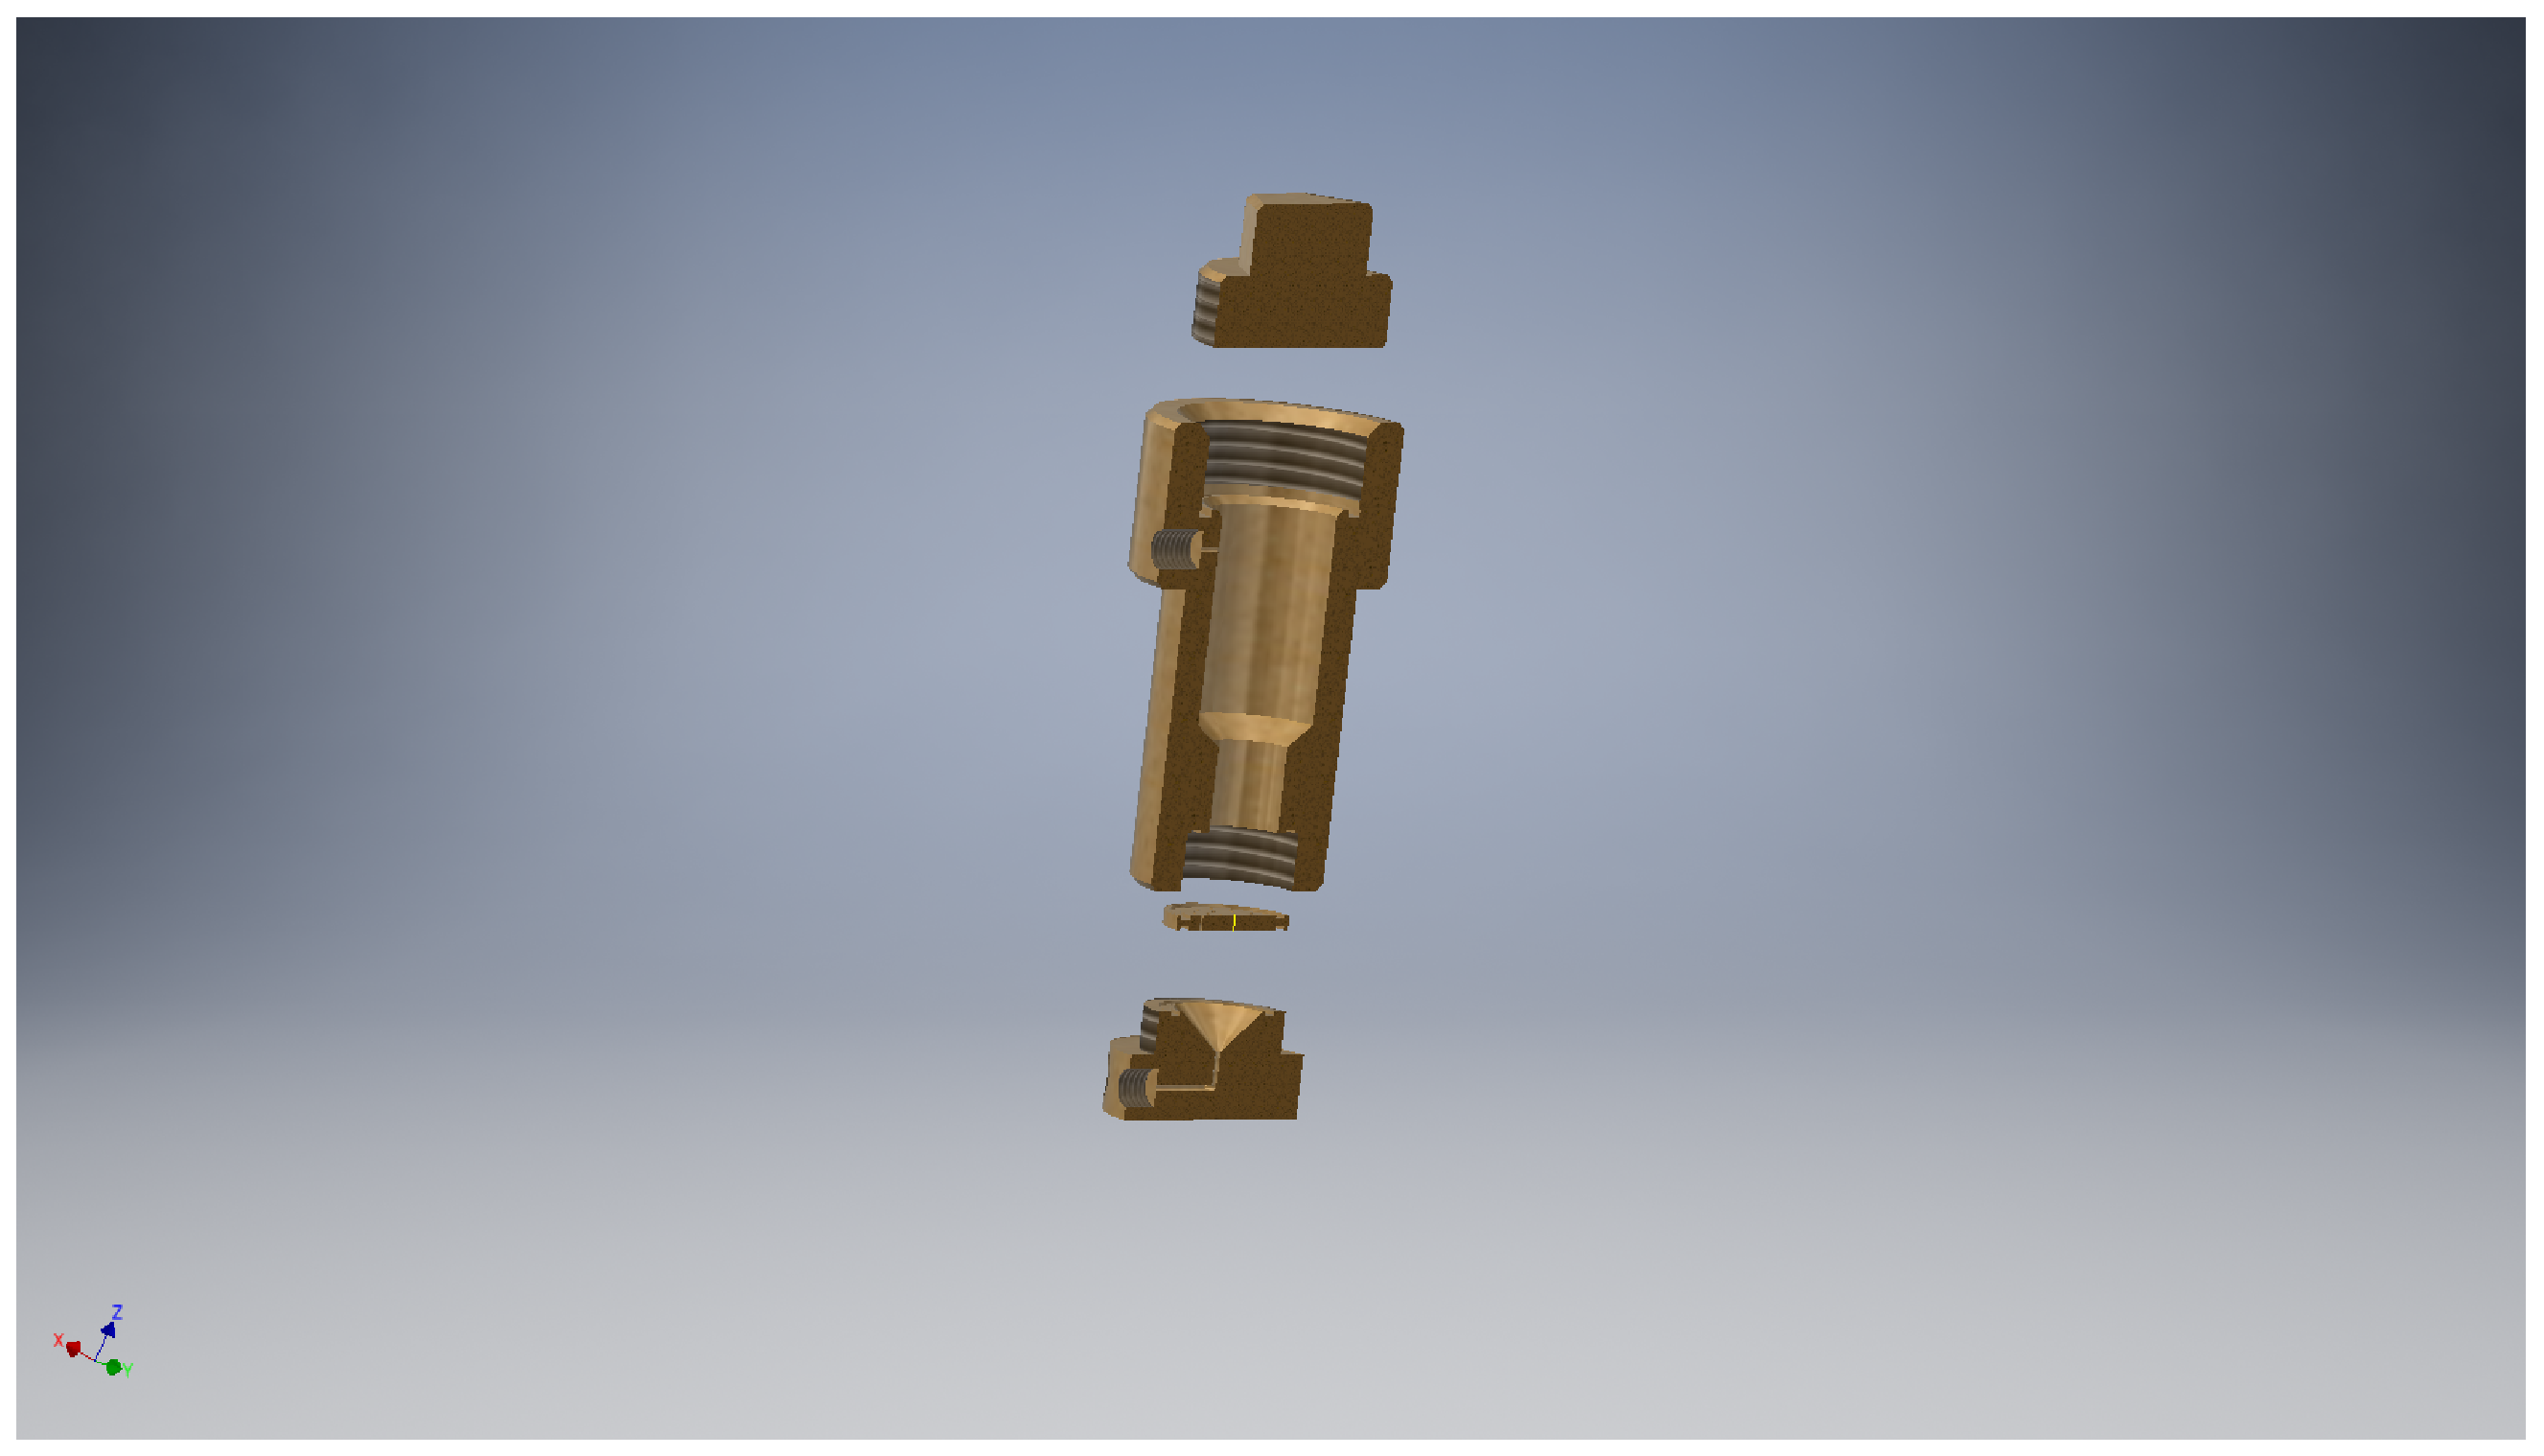
\includegraphics[width=0.49\textwidth]{/figures/materialsMethods/lowFieldReactor.eps}
                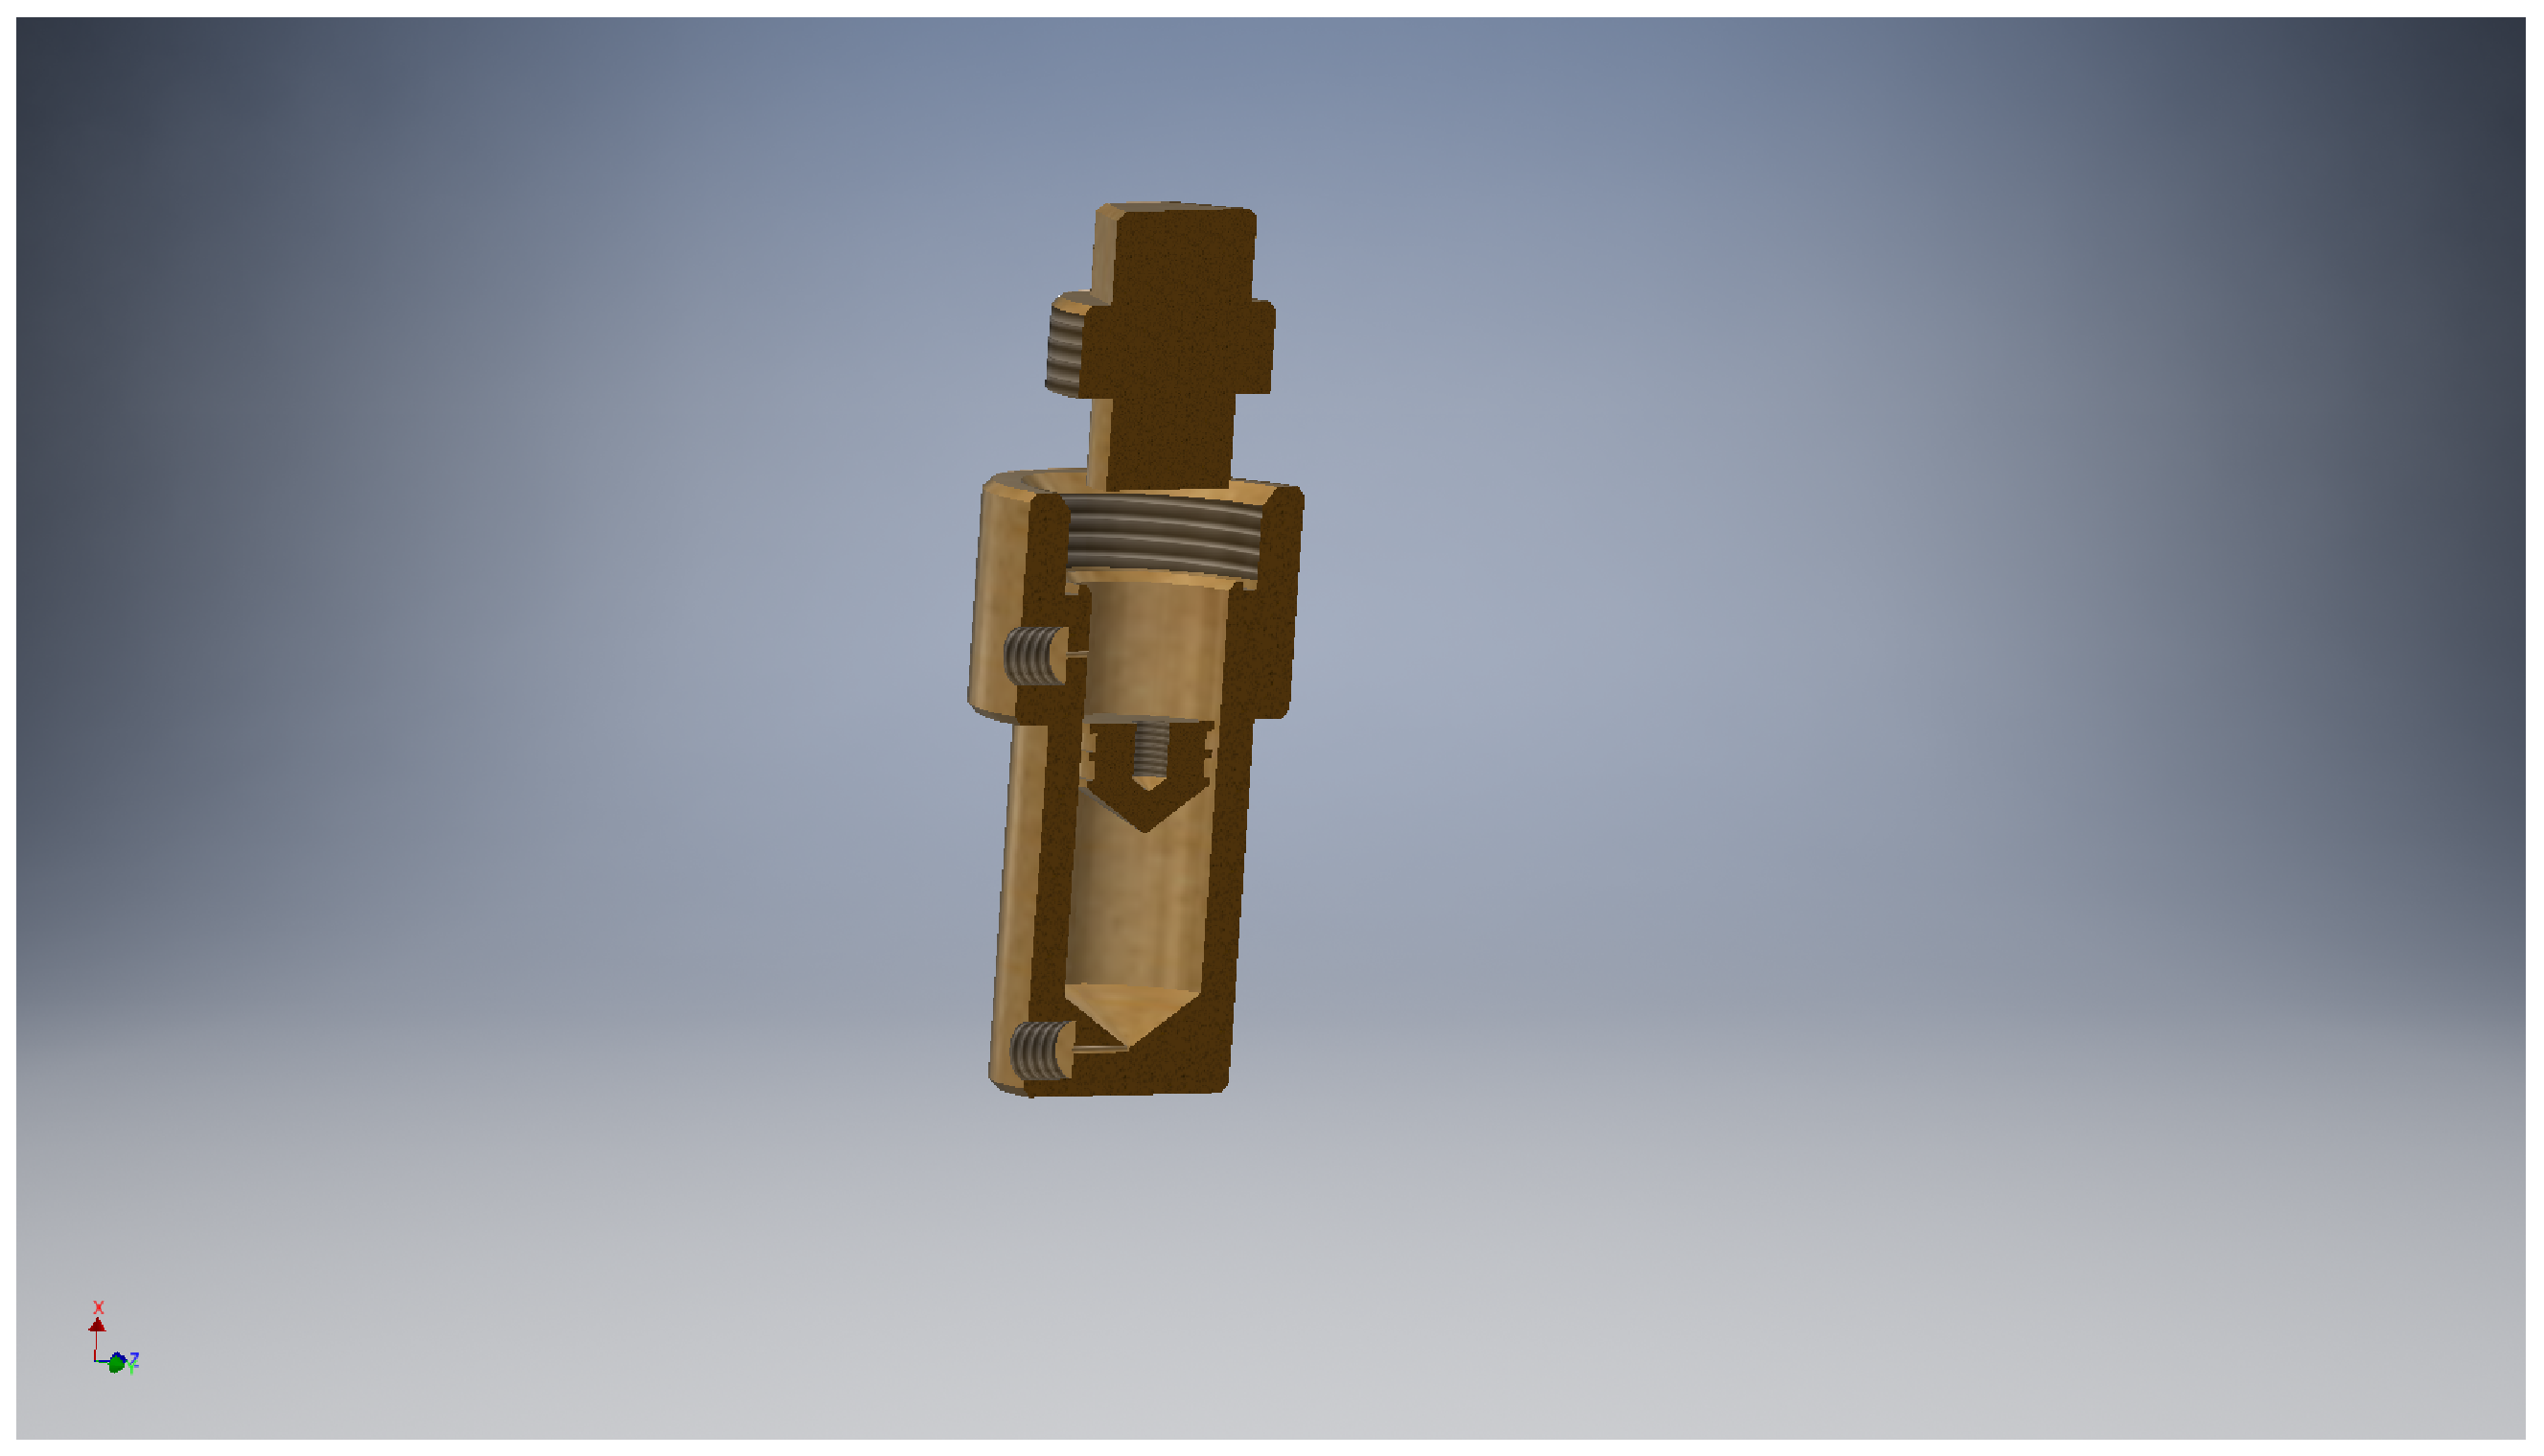
\includegraphics[width = 0.49 \textwidth]{/figures/materialsMethods/highFieldProbe.eps}
                \caption[Reactor gemometry]{Half cut views of the low field reactor (left) and high field probe
                (right). The disk for pH2 provision in the low field reactor is visisble on the bottom sandwiched between the
                main body and the screw on cap. Hose connections are made to that cap and the top
                of the main body. The high field probe is shown with its optional piston inserted,
                the two possible connections at the top for actuation and bottom for sample transfer
                are visible.}
            \end{figure}
        \subsection{High Field Probe}
            Similarly to the one in low field, the high field probe has to withstand the high
            pressures applied and the chemicals used. It is made from the same material, PSU. While
            its conical bottom is similar to the low field probe's, there's no need for a bubbling
            system. There are two procedures for shuttling the solution back to low field: Via a
            piston that can also be actuated by pressurized gas or simply by the gas pressure that
            builds above the solution due to the transfer towards high field. With methanol
            solutions, the latter method turns out to be efficient, other solutions with different
            viscosities may need the piston approach for efficient transport.
        \subsection{Fluid handling system} 
            Sample volumes range in the $\SI{}{\milli\litre}$ regime thus sample losses are
            unfavorable.
    \section{Fluxgate Field Probe}\label{sec:methodsFluxgate}
        \subsection{Arduino Shield}
        As a first test, a shield for a 12 bit arduino microcontroller was built reading out the individual channels on individual analog inputs. Depending on the output voltage, the signal was fed to the analog input unpertubated or split throug a voltage divider if it rose above the analog inputs maximum voltage. The shield was etched in a \todo{acid?} bath after UV-exposure of the light sensitive PCB and development in a \todo{bath}. For exposure, a printed foil bag has been used into which the two sided PCB was inserted  its sides were uv-exposed individually.
        \subsection{Teensy 3.6}
        The alternative solution using a teensy 3.6 microcontroller and a self designed shield provided higher intrinsic bit depth and additional active amplification using operational amplifiers.
%\input{}
